\documentclass[fr]{../../../../../../eplexam}
\usepackage{../../../mmc-MECA1901-exam}
\usepackage{graphicx,amsmath,amssymb}

\hypertitle{Mécanique des milieux continus}{5}{MECA}{1901}{2018}{Janvier}{Majeure}
{Martin Braquet \and Thibault Heremans \and Grégoire van Oldeneel}
{Issam Doghri et Philippe Chatelain}

\section{Théorie (1/2)}

\begin{enumerate}
    \item Soit $\mathrm{dl}=||\mathbf{dX}||$, exprimer 
    \[
        \frac{1}{2}\frac{\mathrm{dl}^2-\mathrm{dL}^2}{\mathrm{dL}^2}
    \]
    en fonction du tenseur $\mathbf{E}$ (exprimé dans la base $\{\mathbf{\hat{e}_1},\mathbf{\hat{e}_2},\mathbf{\hat{e}_3}\}$) pour $\mathbf{dX}$ aligné selon $\mathbf{\hat{e}_1}$  et $\mathbf{dX}$ aligné selon $\mathbf{\hat{e}_1}+\mathbf{\hat{e}_2}$.
    \item Contrainte uniaxiale selon  $\mathbf{\hat{e}_1}$, exprimer l'élongation en fonction du vecteur contrainte de Cauchy et du vecteur de contrainte nominal. Commenter les résultats lorsque l'élongation vaut $\frac{1}{2}$, 1 et 2.
\end{enumerate}

\nosolution

\section{Théorie (2/2)}

\begin{enumerate}
    \item Le théorème de transport de Reynolds s'énonce 
    
    \begin{align*}
        \PTDeriv{}{t}\int_{\Omega(t)}\phi\: \dif v&=\int_{\Omega(t)}\left(\PTDeriv{\phi}{t}+\phi \nabla\cdot\mathbf{v}\right) \: \dif v\\
        &=\int_{\Omega(t)}\fpart{\phi}{t} \:\dif v + \int_{\partial\Omega(t)}\phi(\mathbf{v}\cdot \uni{n})\:\dif s
    \end{align*}
    Interpréter les différents termes et transformer la première relation pour obtenir la seconde. Justifier en énonçant les théorèmes adéquats.
    \item Soit l'expression du tenseur de contrainte d'un solide 
    \[\sigma_{ij}=2\mu\epsilon_{ij}+\lambda \epsilon_{ij}\delta_{ij}-(3\lambda+2\mu)\alpha (T-T_0)\delta_{ij}\]
    \begin{enumerate}
        \item Si ce solide n'est pas libre de se déformer et qu'on élève sa température à $T>T_0$, donner l'expression du champ de contrainte  et l'interpréter.
        \item Inverser cette expression pour donner l'expression du tenseur de déformation en fonction du tenseur des contraintes.
    \end{enumerate}
        
    \item Expliquer brièvement pourquoi il est nécessaire pour un fluide newtonien que les coefficient $\kappa$ et $\mu$ soient positifs.
\end{enumerate}

\begin{solution}
    \begin{enumerate}
    \item Première équation: le premier terme de la somme est la dérivée matérielle du champ $\phi$, c'est-à-dire la variation de ce champ en suivant le point matériel. Le second terme de la somme correspond à une variation de la vitesse associée à ce même point. 
    
    Deuxième équation: il s'agit de la somme de la variation à position fixée et du flux à travers la surface. Pour la résolution, on développe la dérivée particulière, on utilise la définition de dérivée d'un produit, et enfin le théorème de la divergence de Green-Ostrogradski.
    \begin{align*}
        \PTDeriv{}{t}\int_{\Omega(t)}\phi\: \dif v &=\int_{\Omega(t)}\left(\PTDeriv{\phi}{t}+\phi \nabla\cdot\mathbf{v}\right) \: \dif v\\
        &=\int_{\Omega(t)}\left(\fpart{\phi}{t}+ \mathbf{v}\cdot \nabla\phi + \phi\nabla\cdot\mathbf{v}\right) \: \dif v\\
        &=\int_{\Omega(t)}\left(\fpart{\phi}{t}+\nabla \cdot (\phi \mathbf{v}) \right) \: \dif v\\
        &=\int_{\Omega(t)}\fpart{\phi}{t} \: \dif v + \oint_{\partial\Omega(t)}\phi(\mathbf{v}\cdot \uni{n})\:\dif s
    \end{align*}
    
    \item 
        \begin{enumerate}
            \item S'il n'est pas libre de se déformer, c'est que les déformations infinitésimales sont nulles. Pour rappel, $\epsilon_{ii} \triangleq \frac{\norm{\dif x^{(i)}}-\norm{\dif X^{(i)}}}{\norm{\dif X^{(i)}}}$ et $\epsilon_{ij}\triangleq \frac{1}{2}\left( \fpart{u_{i}}{x_{j}}+\fpart{u_{j}}{x_{i}}\right)$. On impose donc que $\epsilon_{ij} = 0$. Il reste uniquement le terme de dilatation thermique. On obtient:
        \begin{align*}
        \sigma_{ij} &=2\mu\epsilon_{ij}+\lambda \epsilon_{ij}\delta_{ij}-(3\lambda+2\mu)\alpha (T-T_0)\delta_{ij}\\
        &= -(3\lambda+2\mu)\alpha (T-T_0)\delta_{ij}\\
        &= -(3\lambda+2\mu)\alpha (T-T_0)\mathbf{I}
        \end{align*}
        Le tenseur de contrainte $\sigma$ est nul à l'exception de ses termes diagonaux qui sont égaux. La diagonale du tenseur de contrainte correspond aux contraintes normales à chaque face.
        \item Il faut une expression qui relie la trace de $\epsilon$ et celle de $\sigma$. On a en effet que la variation de volume peut s'exprimer comme suit:$$\mathrm{tr}(\epsilon) = \epsilon_{kk} = \frac{1-2\nu}{E}\sigma_{kk} = \frac{1}{3\: K}\mathrm{tr}(\sigma) = \frac{1}{3\lambda+2\mu}\mathrm{tr}(\sigma)$$
        En notation matricielle, on peut réécrire l'expression donnée:
    \begin{align*}
        \sigma &= 2\mu \epsilon + \lambda \mathrm{tr}(\epsilon)\mathbf{I} - (3\lambda +2\mu)\alpha (T-T_0)\mathbf{I}\\
        &=  2\mu \epsilon + \lambda \mathrm{tr}(\epsilon)\mathbf{I} - M(T)\mathbf{I}\\
        &= 2\mu \epsilon + \lambda \frac{1-2\nu}{E}\mathrm{tr}(\sigma) \mathbf{I} - M(T)\mathbf{I}
        \end{align*}
        On isole $\epsilon$ et, avec les définitions de $\lambda$, $\mu$ et $K$, on obtient:
        \begin{align*}
        \epsilon &= \frac{\sigma}{2\mu}-\frac{1}{2\mu}\left( \lambda \frac{1-2\nu}{E}\mathrm{tr}(\sigma) \mathbf{I} + M(T)\mathbf{I}\right)\\
        &= \frac{1+\nu}{E}\sigma - \frac{\nu}{E}\mathrm{tr}(\sigma) + \alpha(T-T_0)
        \end{align*}
    \end{enumerate}
    
    \item Il faut respecter le principe d'admissibilité thermodynamique. On doit ainsi respecter l'inégalité de Clausius-Duhem que l'on peut simplifier: $$ 0 \geq \frac{1}{T} \mathbf{q}\cdot \nabla T $$
    Pour garantir cette inégalité, comme $T>0$ et que, par la loi de Fourier, $\mathbf{q} = -k\nabla T$, il faut $k>0$, avec $k$, la conductivité thermique.
    
    En mécanique des fluides, on a: $\nabla \cdot \mathbf{v} = \mathrm{tr}(D) = 0 $ (par conservation de la masse); par ailleurs, on rappelle $I:A = \mathrm{tr}(A)$. On exprime l'inégalité de Clausius-Duhem:
    $$ \rho T \frac{DS}{Dt} - \rho \frac{De}{Dt}\geq \frac{1}{T}\mathbf{q}\cdot \mathbf{\nabla}T - \mathbf{\sigma}:\mathbf{D}$$
    Pour un fluide, on a:
    \begin{align*}
        e &= \int c_v \: \dif T \longrightarrow \fpart{e}{t} = c_v\PTDeriv{T}{t}\\
        S &= \int \frac{c_v}{T} \:\dif T \longrightarrow c_v\PTDeriv{S}{t} = \frac{c_v}{T}\PTDeriv{T}{t}\\
        \sigma &= 2\mu D - pI \longrightarrow \sigma : D = (2\mu D-pI):D = 2\mu D:D
    \end{align*}
    Les deux membres de gauche s'annulent donc mutuellement. Il reste:
    $$2\mu (D:D) + \frac{k}{T}\Delta T \geq 0$$
    Ce qui est garanti si $k\geq 0$ (montré plus haut) ET si $\mu \geq 0$.
    
    \end{enumerate}
    
\end{solution}


\section{Disque comprimé}
Un cercle dans le repère $(O,\mathbf{\hat{e}_1},\mathbf{\hat{e}_2})$ est soumis à 3 cas de charge différents. Pour le premier cas de charge, $\sigma_{11}(0,0) = \frac{P}{\pi R}$ tandis que $ \sigma_{22}(0,0) = \frac{-3P}{\pi R}$. 

\begin{figure}[h]
    \centering
    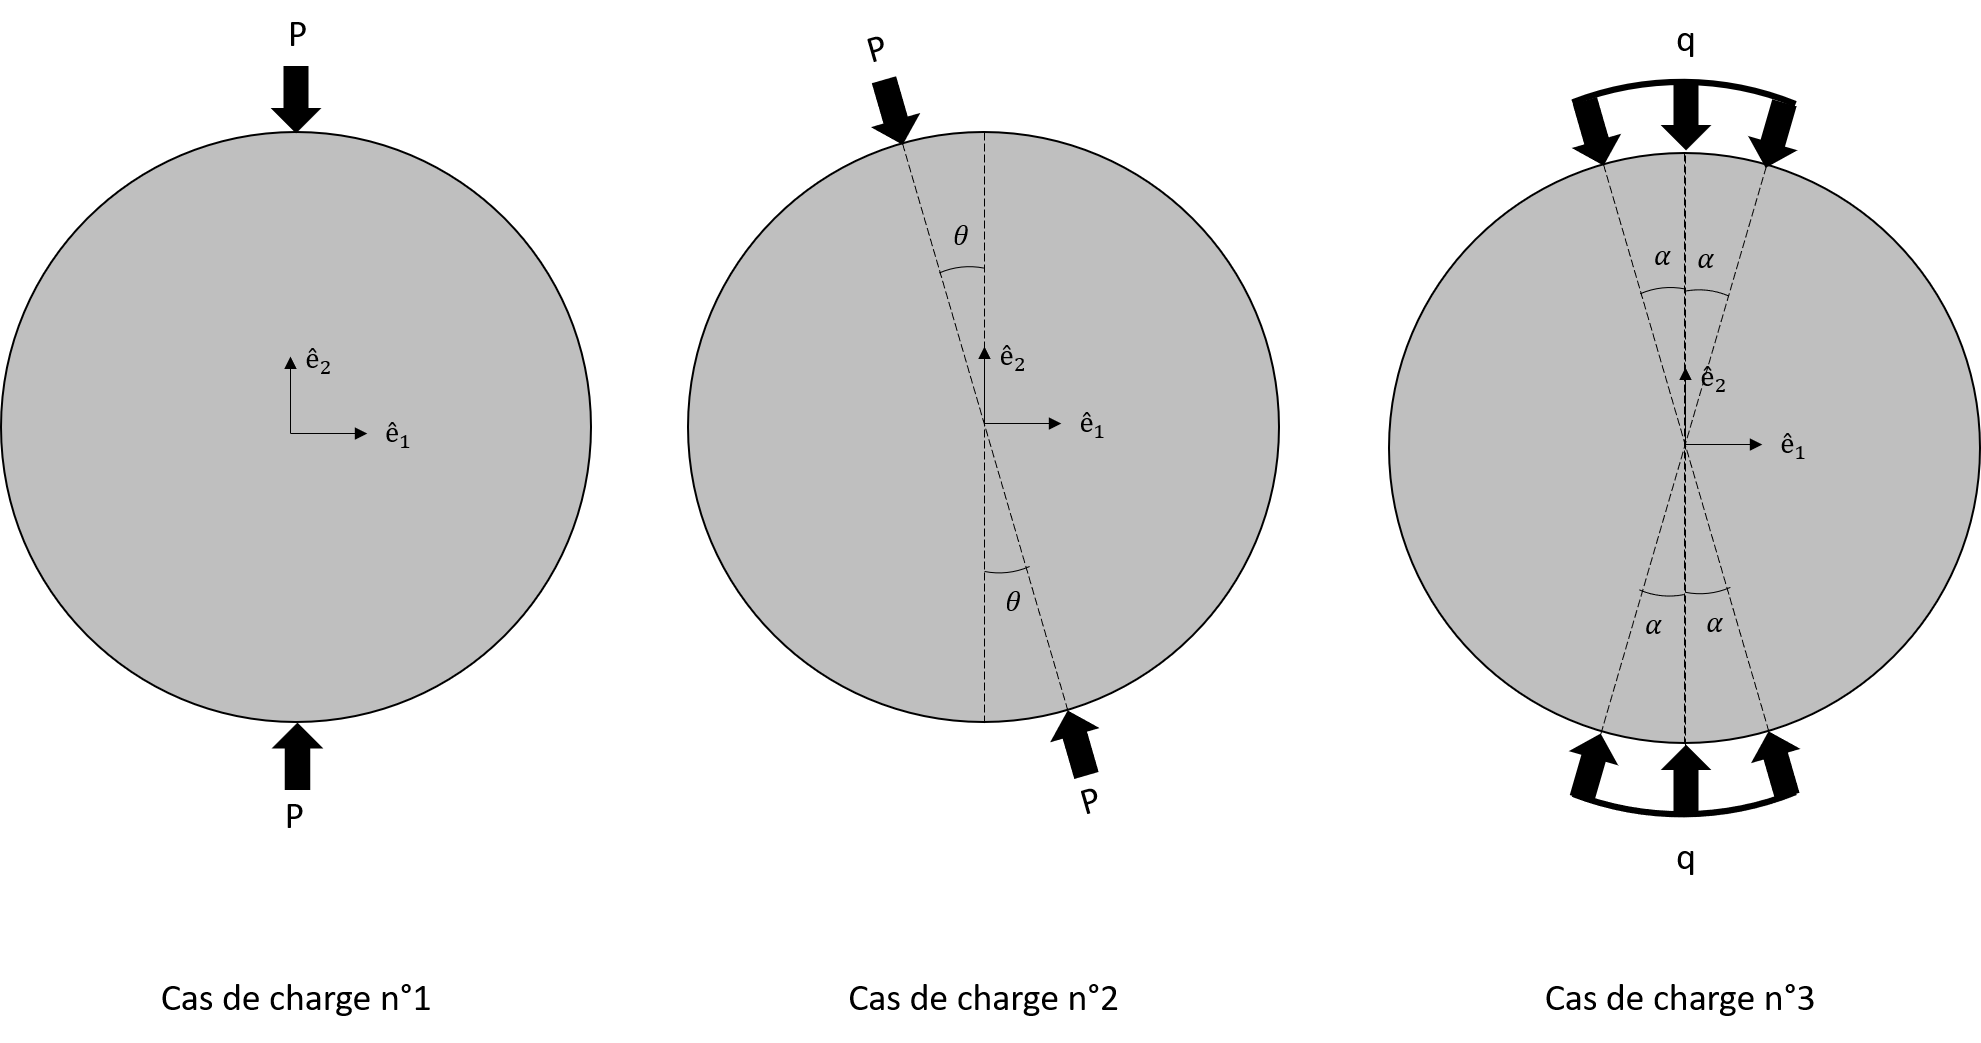
\includegraphics[width=0.9\linewidth]{20181}
\end{figure}


\begin{enumerate}
\subsection*{Cas de charge n\textdegree1}
    \item Représenter (de manière graphique) les contraintes sur un élément matérielle en O dont les normales des faces sont orientées selon (i) $\mathbf{\hat{e}_1}$ et $\mathbf{\hat{e}_2}$ et (ii) si on tourne l'élément matérielle de $\frac{\pi}{4}$.
    %% C'est sûr qu'il demandait aussi lorsqu'on tourne l'élément de pi/4 ?
\subsection*{Cas de charge n\textdegree2}
    \item Exprimer l'état de contrainte en $O$ en fonction de $\theta$.
\subsection*{Cas de charge n\textdegree3}
    \item À partir de l'expression des charges trouvé au second cas et grâce au principe de superposition, déterminer l'expression des contraintes  $\sigma_{11}(0,0) ,\: \sigma_{22}(0,0) ,\: \sigma_{12}(0,0) $.
    \item Si $\alpha=\pi/2$, réexprimer les contraintes et commenter.
    \item Si $\alpha$ tend vers $0$, mais que $\alpha q$ est fini et positif, recalculer les contraintes.
    \item En considérant $P=2q\alpha R$, calculer les contraintes et commenter le résultat.
    \item Tracer les cercles de Mohr. Calculer la contrainte de cisaillement maximale, ainsi que l'angle $\alpha$ pour lequel ce cisaillement maximal se produit.
    
\end{enumerate}

\nosolution

\section{Cylindres coaxiaux poreux}
On considère l'écoulement stationnaire d'un fluide visqueux newtonien entre un cylindre de rayon $\alpha R$ et un cylindre de rayon $R$. Le cylindre de rayon $\alpha R$ et la zone hors du cylindre extérieur (en $r\geqslant R$) sont fixes mais constituées d'un matériaux poreux, le fluide traverse donc perpendiculairement ces parois. On considère les cylindres infinis selon l'axe $z$. De plus, on ajoute un débit surfacique $q_I$ ($[m/s]$) en $r=\alpha R$, qui sort du cylindre intérieur et se dirige vers la zone d'écoulement du fluide. Vu la géométrie du problème, on suppose que le champ de pression est de la forme $p(r,z)=f(r)+g(z)+\mathrm{Cste}$. Il n'y a pas de force à distance (donc pas de force gravitationnelle). Aux extrémités $z=0$ et $z=L$ du cylindre, la pression vaut respectivement $p_0$ et $p_L$ sur la face externe. La longueur du cylindre est beaucoup plus grande que son rayon: $L\gg R$. On suppose également que le champ de vitesse est donné par $\mathbf{v}(r)=v_r(r)\:\Base{r}+v_z(r)\:\Base{z}$. 
On suppose que les propriétés du fluide $\rho,\mu, \kappa$ sont constantes. 


\begin{figure}[h]
    \centering
    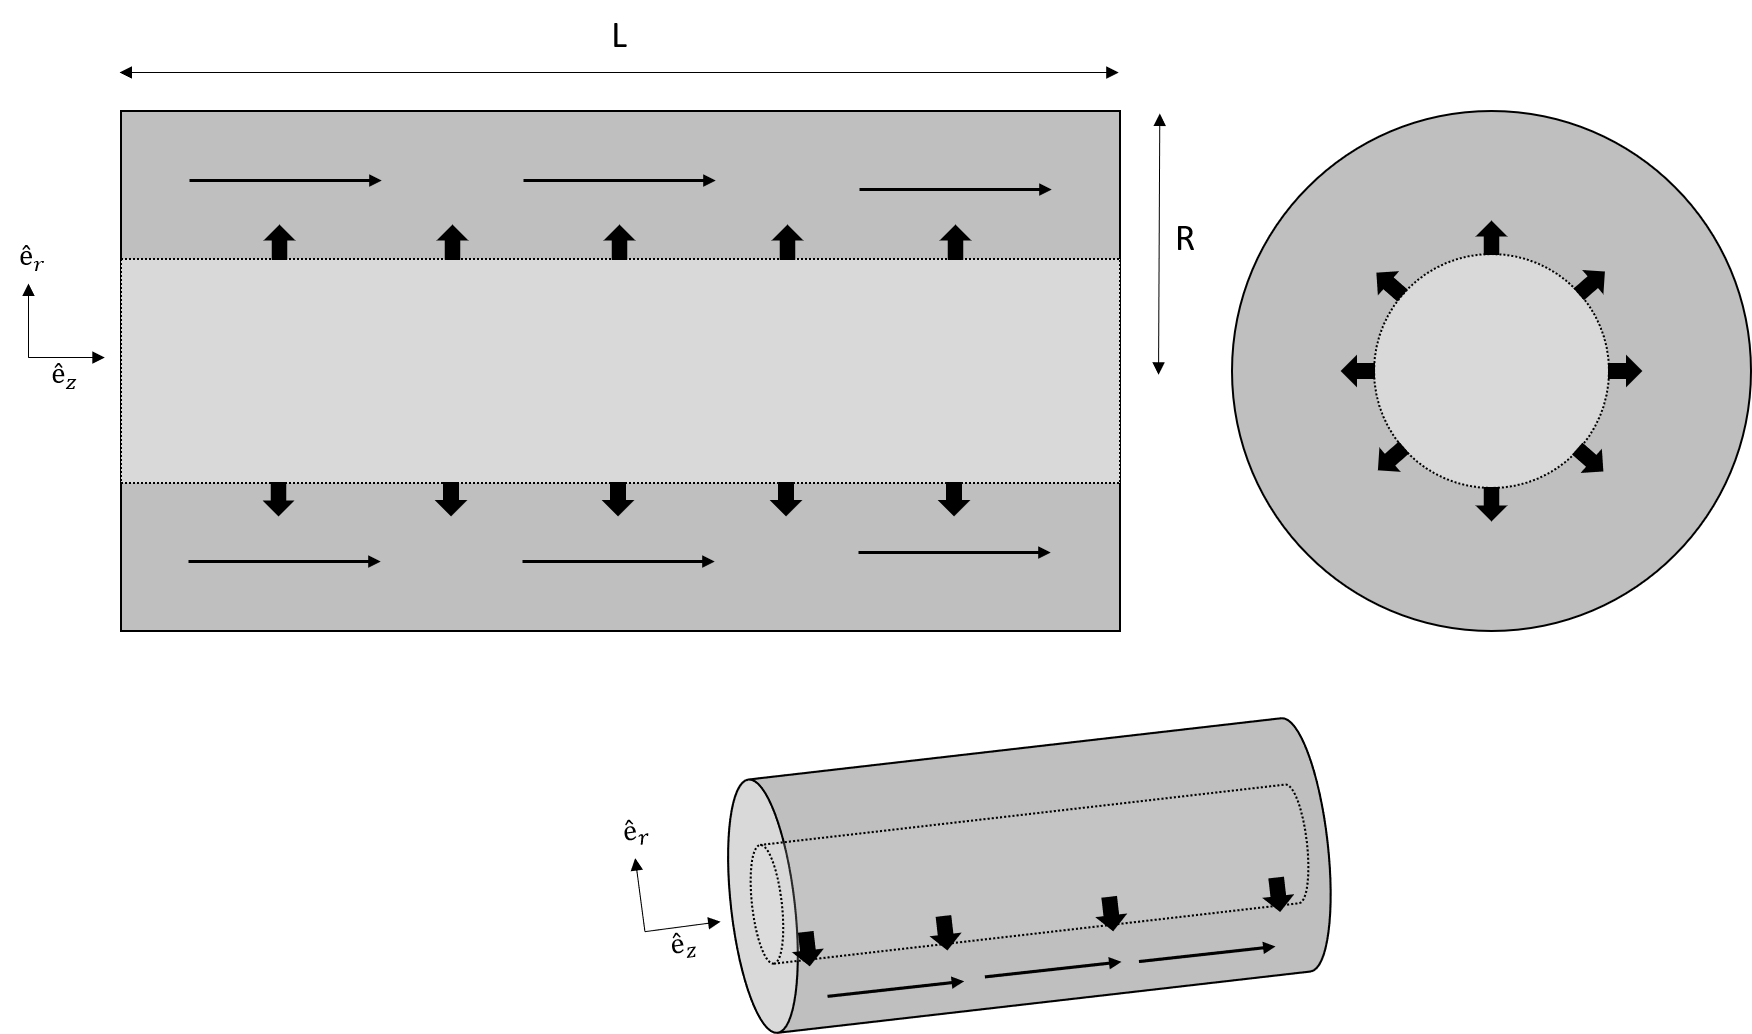
\includegraphics[width=0.7\linewidth]{2018}
\end{figure}


\begin{enumerate}
    \item En partant de l'expression générale d'un champ de vitesse, établir des hypothèses pour montrer que la forme finale du champ de vitesse est bien celle donnée dans l'énoncé.
    \item Montrer que la composante selon $r$ de la vitesse est bien $v_r(r) = \frac{A}{r} $.
    \item Calculer l'expression de la constante $A$.
    \item Résoudre l'équation pour trouver le champ de pression.
    \item La forme de l'expression de la composante du champ de vitesse selon $z$ est de la forme suivante : 
    \[
    v_z(r) = C \left( D - \left(\frac{r}{R}\right)^2 - E \: \frac{1 - \left(\frac{r}{R}\right)^\beta}{1 - \alpha^\beta}\right) 
    \]
    Obtenez l'expression des constantes $C,D$ et $E$ sachant que $\beta$ est une constante et a pour expression : $ \beta = (\rho \: q_I\: \alpha R)/\mu$.
    \item Donner les unités de $\beta$.
    \item Ecrire les équations à résoudre pour établir la trajectoire d'une particule située à la position $(r^*,\theta^*,z^*)$ en $t=0$.
    \item Calculer le temps de transit d'une particule dans la région d'écoulement. 
    \item Démontrer que l'équation de conservation de la quantité de mouvement sous forme globale est conservée pour ce problème.
\end{enumerate}

\begin{solution}

\begin{enumerate}
    \item L'expression générale est donnée par
    \[
        \mathbf{v}(r,\theta,z,t)=v_r(r,\theta,z,t)\:\Base{r}+v_\theta(r,\theta,z,t)\:\Base{\theta}+v_z(r,\theta,z,t)\:\Base{z}
    \]
    Par axisymétrie, l'écoulement est purement axial et radial (terme $v_{\theta}$ nul) et il n'y a pas de dépendance en $\theta$. Le problème ne dépend pas du temps car il est stationnaire. Puisque le fluide est incompressible et que la longueur est considérée infinie , la vitesse selon $z$ est nulle et l'écoulement ne dépend pas de $z$ car l'écoulement est établi.
    
    
    \item Conservation de la masse (Navier-Stokes). $\div \mathbf{v} = 0$, qui est bien vérifiée.
    $$\frac{v_r}{r} + \frac{1}{r} \fpart{v_r}{r} = 0\quad \Longrightarrow \quad v_r(r)=\frac{A}{r} \quad ,A\in \Re$$
    
    
    \item On utilise la condition frontière $v_r(r=\alpha R) = q_I\: \Base{r}$.
    $$\frac{A}{\alpha R} = q_I \quad \Longrightarrow \quad A = \alpha q_I R$$
    
    
    \item Conservation de la quantité de mouvement (Navier-Stokes): $\rho \PTDeriv{\mathbf{v}}{t} = \rho f - \grad p + \mu \Delta \mathbf{v} $. 
    
    Le terme $\rho f$ s'annule puisqu'il n'y a pas de force à distance. On détaille les autres:
    
    \begin{itemize}
        \item $\nabla \mathbf{v} =$ 
        \[ 
            \begin{pmatrix}
            \fpart{v_r}{r} & 0 & \fpart{v_z}{r}\\
            0 & \frac{v_r}{r} & 0 \\
            0 & 0 & 0\\
            \end{pmatrix} 
        \]

        \item $\PTDeriv{\mathbf{v}}{t} = \underbrace{\fpart{\mathbf{v}}{t}}_{0} + \mathbf{v} \cdot \nabla \mathbf{v} =$ 
        $$\begin{pmatrix}
            v_r & 0 & v_z
        \end{pmatrix} $$
        $$\begin{pmatrix}
            \fpart{v_r}{r} & 0 & \fpart{v_z}{r}\\
            0 & \frac{v_r}{r} & 0 \\
            0 & 0 & 0\\
        \end{pmatrix}$$
        $= v_r \fpart{v_r}{r} \Base{r} + v_r \fpart{v_z}{r} \Base{z}$
        
        \item $\nabla p = \fpart{p}{r} \Base{r} + \fpart{p}{z}\Base{z} = f'(r) \:Base{r} + g'(z)\: \Base{z}$
        
        \item $\Delta \mathbf{v} = \left( \Delta v_r - \frac{v_r}{r^2} \right)\: \Base{r} +( \Delta v_z)\: \Base{z} = \left(\ffpart{v_r}{r} + \frac{1}{r} \fpart{v_r}{r} - \frac{v_r}{r^2} \right) \:\Base{r} + \left( \ffpart{v_z}{r} + \frac{1}{r} \fpart{v_z}{r} \right)\: \Base{z}$
        
    \end{itemize}
    
    Cela fait donc les 3 équations suivantes à satisfaire :
    \begin{align}
        \rho v_r \fpart{v_r}{r} &= - f'(r) + \mu \left(\ffpart{v_r}{r} + \frac{1}{r} \fpart{v_r}{r} - \frac{v_r}{r^2} \right)\\
        0 &= 0\\
        \rho v_r \fpart{v_z}{r} &= - g'(z) +\mu \left( \ffpart{v_z}{r} + \frac{1}{r} \fpart{v_z}{r} \right)
    \end{align}
    
    L'équation (3) peut se réécrire comme $g'(z) = h(r) = F$ par séparation de variable, ce qui permet de trouver l'expression de $g(z)$.
    $$g(z) = Fz + D$$
    
    Reprenons l'équation (1). Le terme multiplié par $\mu$ s'annule : $\Big( \frac{2A}{r^3} - \frac{1}{r}\frac{A}{r^2} - \frac{1}{r^2}\frac{A}{r}\Big) = 0$. Il nous reste alors :
    $$f'(r) = -\rho v_r \fpart{v_r}{r} = \rho \frac{A^2}{r^3} $$
    $$f(r) = - \rho \frac{A^2}{2 r^2} = -\rho \frac{\alpha^2 q_I^2 R^2}{2 r^2}$$
    
    On peut alors maintenant rassembler les différents termes de $p$ et appliquer les conditions frontières.
    
    $$p(r,z) = Fz - \rho \frac{A^2}{2 r^2} + D = Fz -\rho \frac{\alpha^2 q_I^2 R^2}{2 r^2}+  D$$
    
    La première condition $p(R,0)=p_0$ implique que $D=\rho \frac{\alpha^2 q_I^2}{2}+p_0$.
    
    La seconde condition sur le champ de pression, $p(R,L)=p_L$ implique $F=\frac{p_L-p_0}{L}$.
    La pression est ainsi déterminée:
    \[
        p(r,z)=p_0+(p_L-p_0)\frac{z}{L}+\frac{1}{2}\rho\alpha^2 q^2\left( 1-\left( \frac{R}{r}\right)^2\right)
\]
    \item 
    Puisque la vitesse du fluide est normale aux parois à ses extrémités, la composante axiale de la vitesse est nulle sur les parois: $v_z(r=\alpha R)=v_z(r=R)=0$.
    \[
        v_z(r=R)=C(D-1)=0\quad\Longrightarrow\quad D=1
    \]
    \[
        v_z(r=\alpha R)=C(D-\alpha^2-E)=0\quad\Longrightarrow\quad E=1-\alpha^2
    \]
    Pour trouver la dernière constante $C$, on utilise l'équation (3):
    \begin{align*}
        F&=-\rho v_r \fpart{v_z}{r} +\mu \left( \ffpart{v_z}{r} + \frac{1}{r} \fpart{v_z}{r} \right)\\
        F&=\mu \ffpart{v_z}{r}+\left(\frac{\mu}{r}-\rho \frac{A}{r}\right) \fpart{v_z}{r}\\
        F&=\mu C\left(-\frac{2}{R^2}+\frac{\beta(\beta-1) E}{R^\beta}\frac{r^{\beta-2}}{1 - \alpha^\beta}\right) + \left(   \frac{\mu}{r}-\rho \frac{A}{r}\right)C\left(-\frac{2r}{R^2}+\frac{\beta E}{R^\beta}\frac{r^{\beta-1}}{1 - \alpha^\beta}\right)\\
        F&=-\frac{2\mu}{R^2}C+\mu\frac{\beta(\beta-1) E}{R^\beta}\frac{r^{\beta-2}}{1 - \alpha^\beta}C -\frac{2\mu}{R^2}C+\frac{2\rho A }{R^2}C+\frac{\beta E}{R^\beta}\frac{r^{\beta-2}}{1 - \alpha^\beta}\left(\mu-\rho A\right)C\\
        F&=\left(2\rho A -4\mu\right)\frac{C}{R^2}+\frac{ E}{R^\beta} \frac{ r^{\beta-2}}{1 - \alpha^\beta}\Big(\mu\beta(\beta-1)+(\mu-\rho A)\beta \Big)C
    \end{align*}
    Comme cette relation est valable pour tout $r\in[\alpha R;R]$, il faut que:
    \[
        F=\left(2\rho A -4\mu\right)\frac{C}{R^2}\quad\Longrightarrow\quad C=\frac{1}{2}\frac{R^2 F}{\rho A -2\mu}=\frac{1}{2}\frac{R^2}{\rho q_I\alpha R -2\mu}\frac{p_l-p_0}{L}
    \]
    et 
    \[
        \mu\beta(\beta-1)+(\mu-\rho A)\beta=0 \quad\Longrightarrow\quad \beta=\frac{\rho A}{\mu}=\frac{\rho q_I\alpha R}{\mu}
    \]
    Cette dernière relation est bien celle qui est donnée dans l'énoncé.

    \item $\beta$ est adimensionnel car il est en exposant. On peut le confirmer par les unités de son expression donnée dans l'énoncé:

        $$[\beta] = \frac{kg}{m^3} \frac{m}{s}m \frac{m s}{kg} = [/]  $$
        
        Pour retrouver les unités de $\mu$, on regarde sur le formulaire et on voit que les unités de $\mu \mathbf{D}$ doivent valoir les unités de $\pmb{\sigma}$. $\mathbf{D}$ est en $s^{-1}$ et $\pmb{\sigma}$ en $\frac{N}{m^2}=\frac{kg}{s^2 m}$.


    \item Le problème est stationnaire donc les trajectoires, lignes d'émissions et de courant se confondent. On doit résoudre le problème de Cauchy suivant :
    
    \[
        \dif \mathbf{x} = \mathbf{v}(r) \:\dif t\quad\Longrightarrow\quad \left\{ \begin{array}{rcl} \dif r&=&v_r(r)\: \dif t \\ r\:\dif \theta&=&0 \\ \dif z&=&v_z(r)\: \dif t \end{array} \right.\quad\Longrightarrow\quad \left\{ \begin{array}{rcl} \dif r&=&\frac{A}{r}\: \dif t \\ \dif \theta&=&0 \\ \dif z&=&v_z(r)\: \dif t \end{array} \right.
    \]
    avec $\mathbf{x}(t=0)=(r^*,\theta^*,z^*)$.
    
    On résoud les deux premières équations:
    \[
        \left\{ \begin{array}{rcl} r(t)&=&\sqrt{(r^*)^2+2At} \\ \theta(t)&=&\theta^* \\ dz&=&C \left( D - \left(\frac{r(t)}{R}\right)^2 - E \: \frac{1 - \left(\frac{r(t)}{R}\right)^\beta}{1 - \alpha^\beta}\right) \: \dif t \end{array} \right.
    \]
    La dernière équation peut se résoudre en remplaçant $r(t)$:
    \[
        \dif z=C \left( D - \frac{(r^*)^2+2At}{R^2} - E \: \frac{1 - \frac{1}{R^\beta}\left((r^*)^2+2At\right)^{\beta/2}}{1 - \alpha^\beta}\right) \: \dif t
    \]
    On ne fait pas l'intégrale car elle ne l'est pas demandée.
    \item Il faut déterminer le temps mis par une particule pour traverser la zone d'écoulement, c'est donc la vitesse radiale qui influence uniquement ce déplacement. Soit $t^*$, le temps nécessaire, on doit résoudre
    \[
        r(t^*) = \sqrt{(r^*)^2+2At^*}
    \]
    avec $r^*=\alpha R$ et $r(t^*)=R$. Le temps de transit vaut donc
    \[
        t^*=\frac{R^2}{2A}(1-\alpha^2)=\frac{R}{2\alpha q_I}(1-\alpha^2)
    \]
    
    \item 
    L'équation de conservation de la quantité de mouvement s'écrit
    \[
        \mathbf{F}=\fdif{}{t}\int_{\Omega(t)} \rho \mathbf{v}\: \dif v+\oint_{\partial\Omega(t)}\rho \mathbf{v}\:(\mathbf{v}-\mathbf{v_s})\cdot \uni{n}\: \dif s
    \]
    On considère un volume de contrôle fixe allant de $r=\alpha R$ à $r=R$ et de $z=0$ à $z=L$. Sans force de volume et pour un problème stationnaire, elle se simplifie en
    \[
        \oint_{\partial\Omega(t)}\mathbf{t}\:\dif s=\int_{S_i}\rho \mathbf{v}\:\mathbf{v}\cdot \uni{n}\: \dif s+\int_{S_e}\rho \mathbf{v}\:\mathbf{v}\cdot \uni{n}\: \dif s+\int_{S_0}\rho \mathbf{v}\:\mathbf{v}\cdot \uni{n}\: \dif s+\int_{S_L}\rho \mathbf{v}\:\mathbf{v}\cdot \uni{n}\: \dif s
    \]
    où $S_i,S_e,S_0$ et $S_L$ désignent respectivement les surfaces interne (en $r=\alpha R$), externe (en $r=R$), inférieure (en $z=0$) et supérieure (en $z=L$).
    Les forces de contact valent
    \[
        \int_{\partial\Omega(t)}\mathbf{t}\:\dif s=\int_{S_0}p(r,0)\:\Base{z}\:\dif s+\int_{S_L}-p(r,L)\:\Base{z}\:\dif s+\int_{S_i}p(\alpha R,z)\:\Base{r}\:\dif s+\int_{S_e}-p(R,z)\:\Base{r}\:\dif s
    \]
    Les deux premiers termes valent
    \begin{align*}
        \int_{S_0}p(r,0)\:\Base{z}\:\dif s+\int_{S_L}-p(r,L)\:\Base{z}\:\dif s&=\int_{\alpha R}^R 2\pi r\: p(r,0)\:\dif r\:\Base{z}-\int_{\alpha R}^R 2\pi r\: p(r,L)\:\dif r\:\Base{z}\\
        &=\int_{\alpha R}^R 2\pi r\: \Big(p(r,0)-p(r,L)\Big)\:\dif r\:\Base{z}\\
        &=\int_{\alpha R}^R 2\pi r\: (p_0-p_L)\:\dif r\:\Base{z}\\
        &=\pi R^2(p_0-p_L)(1-\alpha^2)\:\Base{z}\\
    \end{align*}
    et les deux derniers termes valent
    \begin{align*}
        \int_{S_i}p(\alpha R,z)\:\Base{r}\:\dif s+\int_{S_e}-p(R,z)\:\Base{r}\:\dif s&=\int_{0}^L \alpha R \:p(\alpha R,z)\:\dif z\:\int_0^{2\pi}\Base{r}\:\dif \theta-\int_{0}^L R \:p(R,z)\:\dif z\:\int_0^{2\pi}\Base{r}\:\dif \theta\\
        &=0
    \end{align*}
    On détaille le membre de droite:
    \begin{align*}
    \int_{S_i}\rho \mathbf{v}\:\mathbf{v}\cdot \uni{n}\: \dif s+\int_{S_e}\rho \mathbf{v}\:\mathbf{v}\cdot \uni{n}\: \dif s&=\alpha R\int_0^{2\pi}\int_{0}^L\rho \mathbf{v}\:\mathbf{v}\cdot (-\Base{r})\: \dif \theta\:\dif z+ R\int_0^{2\pi}\int_{0}^L\rho \mathbf{v}\:\mathbf{v}\cdot \Base{r}\:\dif \theta\: \dif z\\
    &=- \alpha R\int_0^{2\pi}\int_{0}^L\rho \mathbf{v}(\alpha R)\:v_r(\alpha R)\: \dif \theta\: \dif z+ R\int_0^{2\pi}\int_{0}^L\rho \mathbf{v}(R)\:v_r(R)\: \dif \theta\: \dif z\\
    &=- \alpha R\int_{0}^L\rho v_r(\alpha R)\: \dif z\int_0^{2\pi}\:\frac{A}{\alpha R}\Base{r}\:\dif \theta + R\int_{0}^L\rho v_r(R)\: \dif \theta\: \dif z\int_0^{2\pi}\:\frac{A}{ R}\Base{r}\:\dif \theta \\
    &=0
    \end{align*}
    Les deux derniers termes du membre de droite sont égaux à
    \begin{align*}
    \int_{S_0}\rho \mathbf{v}\:\mathbf{v}\cdot \uni{n}\: \dif s+\int_{S_L}\rho \mathbf{v}\:\mathbf{v}\cdot \uni{n}\: \dif s&=\int_0^{2\pi}\int_{\alpha R}^R\: \rho \mathbf{v}\:\mathbf{v}\cdot \Base{z}\:r\dif \theta\:\dif r+\int_0^{2\pi}\int_{\alpha R}^R\: \rho \mathbf{v}\:\mathbf{v}\cdot (-\Base{z})\:r\dif \theta\:\dif r\\
    &=\int_0^{2\pi}\int_{\alpha R}^R\:\rho \mathbf{v}(r)\:v_z(r)\:r\dif \theta\:\dif r-\int_0^{2\pi}\int_{\alpha R}^R\: \rho \mathbf{v}(r)\:v_z(r)\:r\dif \theta\:\dif r\\
    &=0
    \end{align*}
    car $\mathbf{v}$ est identique en $z=0$ et en $z=L$.
    
    Donc, il y a une erreur dans le raisonnement\dots
\end{enumerate}

\end{solution}

\end{document}
